\documentclass[12pt,a4paper]{article}

\usepackage{jyw-program}

\begin{document}
\title{ITSA-58 參考解答}
\author{Jia-Yin Wang}
\maketitle

\begin{abstract}
這份講義提供ITSA-58競賽的參考解答,主要是給同學做為學習參考之用。基本上這些題目從淺入深,對於初學者來說,後面的題目可能相當困難,所以同學可以根據自己的情況,看能學到哪裡就學到哪裡,不懂的話也沒有關係。只要慢慢學習下去,將來有一天也可以融會貫通。

另外這裡所提供的參考解答,主要是從初學者容易理解的方式來尋找可行的辦法。基本上解決一個問題,常常有很多種可能的方式,所以還是要鼓勵同學繼續學習更多程式的技巧和演算方法,以後可能就會找到其他更好的解法。

學習程式務求完全理解,最好還能實際上機測試,否則好像看過看懂,實際上在作答或應用的時候,還是沒有辦法寫得出來。希望同學在閱讀的同時,可以多加思考,並且實際上機測試,以求完全了解。
\end{abstract}
\newpage
\section{ITSA-58-1 計算正整數被3整除之數值之總和}
\centerline{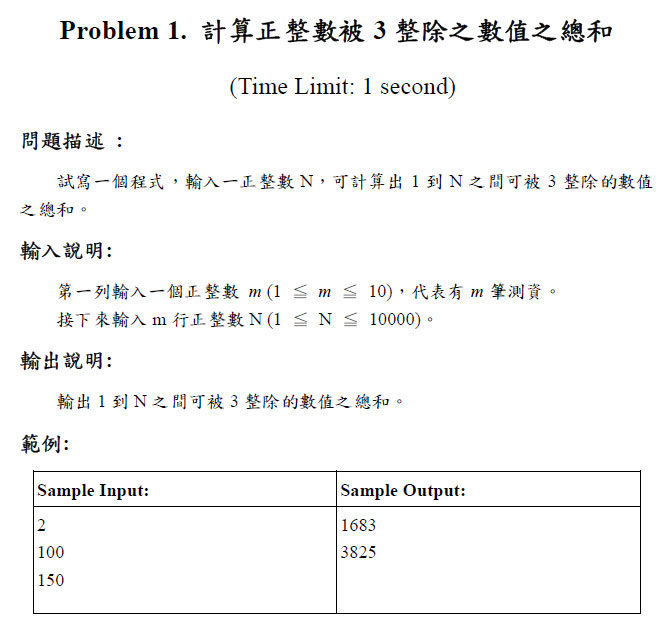
\includegraphics[width=.8\textwidth]{../solutions/fig/58ITSA1}}
\subsection{解題思惟}
\begin{enumerate}
	\item 如果有n個case要處理的話,可以設一個變數,例如kase,讀入n之後,用以下迴圈求解,剛好會跑n次。
	\begin{inside}
		int kase; cin >> kase;
		while (kase--) {
			// 處理一個case
		}
	\end{inside}
	\item 求和的話,可以設一個變數,例如sum=0,然後把要加的都加到sum裡面。
	\item 從1檢查到n的話,可以跑一個for迴圈,像下面這樣:
	\begin{inside}
		for (int i=1; i<=n; i++) {
			// 處理i的情況
		}
	\end{inside}
	\item 檢查i是否為3的倍數,就把i除以3看餘數是否為0,是0的話,i就是3的倍數。
	\begin{inside}
		if (i%3==0) sum += i; // i是3的倍數
	\end{inside}
\end{enumerate}
\subsection{程式碼}
\begin{cppcode}
#include <iostream>

using namespace std;

int main()
{
	int kase, n; cin >> kase;
	while (kase--) {
		cin >> n;
		int sum = 0;
		for (int i=1; i<=n; i++) {
			if (i%3==0) sum += i;
		}
		cout << sum << endl;
	}
	return 0;
}
\end{cppcode}

\newpage
\section{ITSA-58-2 道路修補}
\centerline{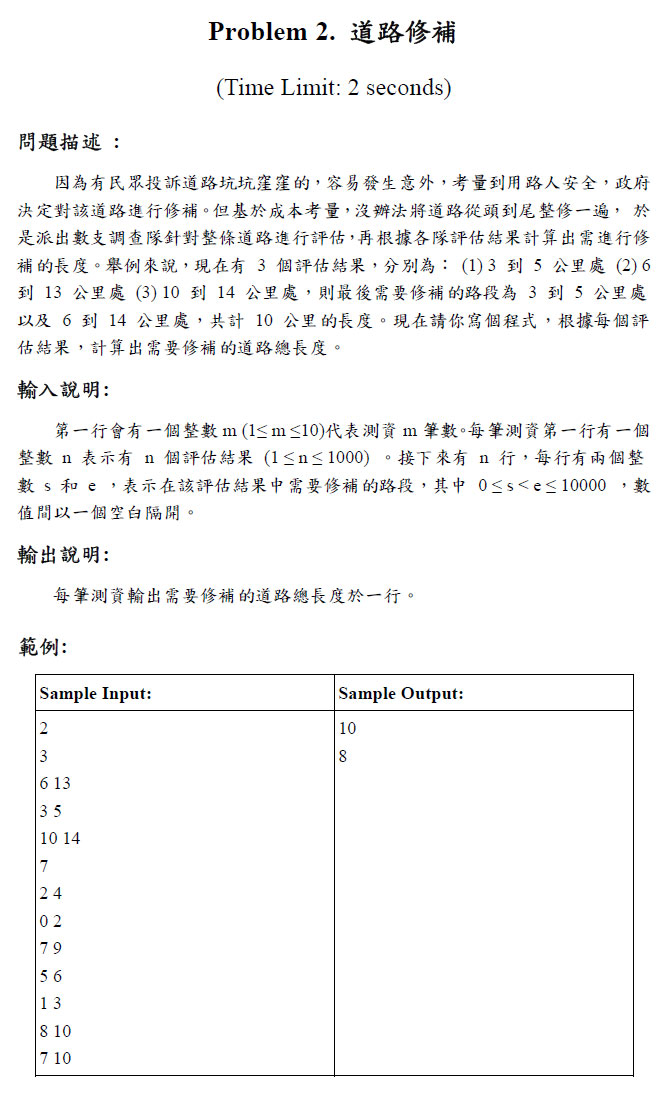
\includegraphics[height=.95\textheight]{../solutions/fig/58ITSA2}}

\subsection{解題思惟}
\begin{enumerate}
	\item m個case的情理方式,同第1題。每個case又有n個評估結果,這個處理方式也相同。
	\item 每一個評估結果,都會輸入s和e,等於是一個線段。最後要求的,其是就是所有n個線段聯集的長度。要怎麼處理聯集的長度呢?
	\item 題目有限制最大的e值不超過10000,那我們可以用一個很簡單的方式來處理,就是直接記錄每一個單位長度i到i+1是否被包含在聯集裡,這樣的話,最多也只有10000個單位線段,那我們可以設一個10000個元素以上的陣列lend,如果線段i到i+1被包含在聯集裡,我們就設lend[i]=1,如果不包含在聯集裡,就設lend[i]=0。最後要求聯集的長度,就把陣列所有元素加總就可以了。
	\item 換一個角度思考,我們可以先把陣列所有元素都設為0,那當我們讀入一個線段[s,e]的時候,直接把lend[s]一直到lend[e-1]全部設為1就可以了。
\end{enumerate}

\subsection{程式碼}
\begin{cppcode}
#include <iostream>

using namespace std;

int main()
{
	int kase, n, s, e, lend[10000];
	while (kase--) {
		for (int i=0; i<10000; i++) lend[i]=0;
		cin >> n;
		while (n--) {
			cin >> s >> e;
			for (int i=s; i<e; i++) lend[i]=1;
		}
		int sum = 0;
		for (int i=0; i<10000; i++) sum+=lend[i];
		cout << sum << endl;
	}
	return 0;
}	
\end{cppcode}
\newpage
\section{ITSA-58-3 完整二元樹}
\centerline{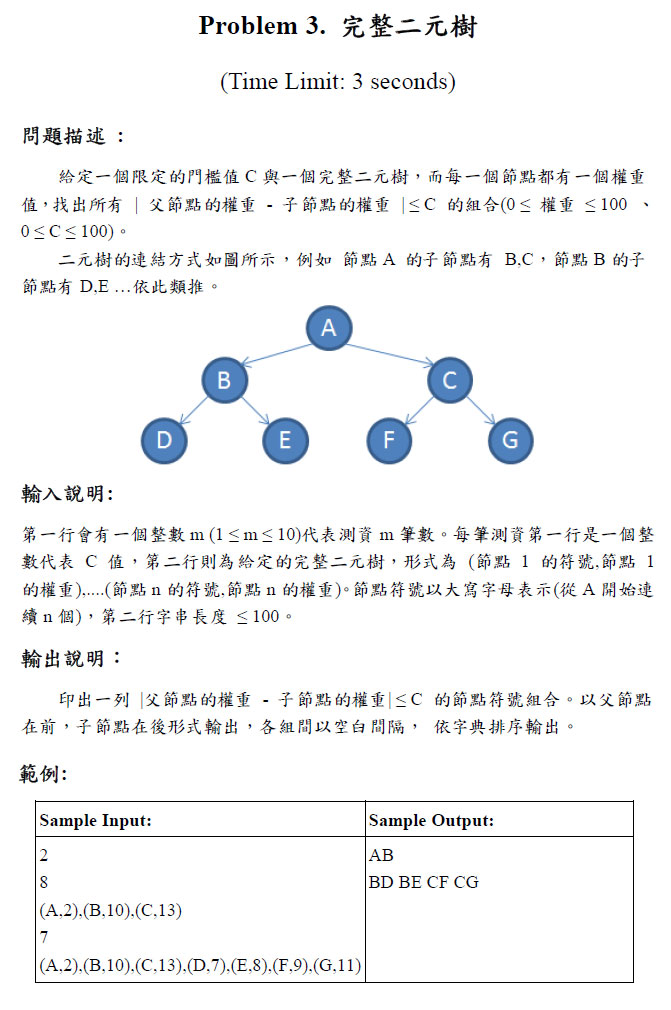
\includegraphics[height=.95\textheight]{../solutions/fig/58ITSA3}}

\subsection{解題思惟}
\begin{enumerate}
	\item $n$層的完整二元樹的節點總共有$2^n-1$個。如果我們從最上層依次從1往下編號的話,仔細檢查,會發現節點$n$的子節點分別是$2n$和$2n+1$。
	\item 讀入的資料,ABC...是依照順序來的,那節點編號也是依次來的,所以其實ABC這些字元可以不用管它,因為節點$i$對應的字元會是'A'+$i-1=64+i$。
	\item 所以我們只要能夠依次讀入$2^n-1$個權重數字到陣列就可以了,假設權重陣列為treeW,接著就是檢查父節點和兩個子節點的權重差距是否在設定的範圍之內,也就是treeW[i]和treeW[2*i]的差以及treeW[i]和treeW[2*i+1]的差是否小於等於C。
	\item 讀入資料的部份怎麼處理呢?首先,每一個case會有幾個節點是不知道的,給定的格式就是用換行結尾的,那如果我們依次讀取字元,等檢查到換行符號的時候,就表示這個case所有的資料都讀完了。要注意的是,如果我們使用scanf來讀取字元,那麼換行符號也會讀到,但如果使用\cc{}來讀取字元,預設的狀況是會忽略空白類的字元,所以會讀不到換行字元,如果要在\cc{}裡面讀到空白字元的話,要先使用以下指令,告訴編譯器不要忽略空白:
	\begin{inside}
		cin >> noskipws;
	\end{inside}
	反之,如果要回到預設忽略空白的情況,則使用以下指令:
	\begin{inside}
		cin >> skipws;
	\end{inside}
	\item 每一組資料都是從左括號開始,如果沒有碰到左括號,我們可以一直讀取字元並把它忽略,讀到左括號之後,後面就是節點字元和它的權重了。接下來我們看一下資料格式,數字一定是在「,」之後,那我們可以繼續一直讀取字元,直到出現「,」為止,碰到「,」之後,接下來就可以直接讀進一個權重數字。
\end{enumerate}
\subsection{程式碼}
\begin{cppcode}
#include <iostream>

using namespace std;

int main()
{
	int kase, C, treeW[105];
	char ch;
	cin >> kase;
	while (kase--) {
		cin >> C;
		int index = 1;
		cin >> skipws; // 一開始不會是換行字元,先忽略空白
		while ((cin>>ch) && (ch!='\n')) { // 進字元迴圈後,以換行結束
			cin >> noskipws; // 進字元迴圈後,不能忽略空白
			if (ch!='(') continue; // 不是左括號,回上面繼續讀
			while ((cin>>ch) && (ch!=',')) ; // 一直讀到「,」為止
			cin >> treeW[index++]; // 讀進權重
		}
		bool first = true; // 這是用來處理輸出各組間空白用的
		for (int p=1; p<index/2; p++) {
			for (int child=2*p; child<2*p+2; child++) {
				int diff = treeW[p] - treeW[child];
				if (diff>=-C && diff<=C) { // 差的絕對值<=C
					if (first) first = false;
					else cout << " "; // 不是第一組的話,先印空白
					cout << (char)(64+p) << (char)(64+child);
				}
			}
		}
		cout << endl;
	}
	return 0;
}
\end{cppcode}
\newpage
\section{ITSA-58-4 購物商圈}
\centerline{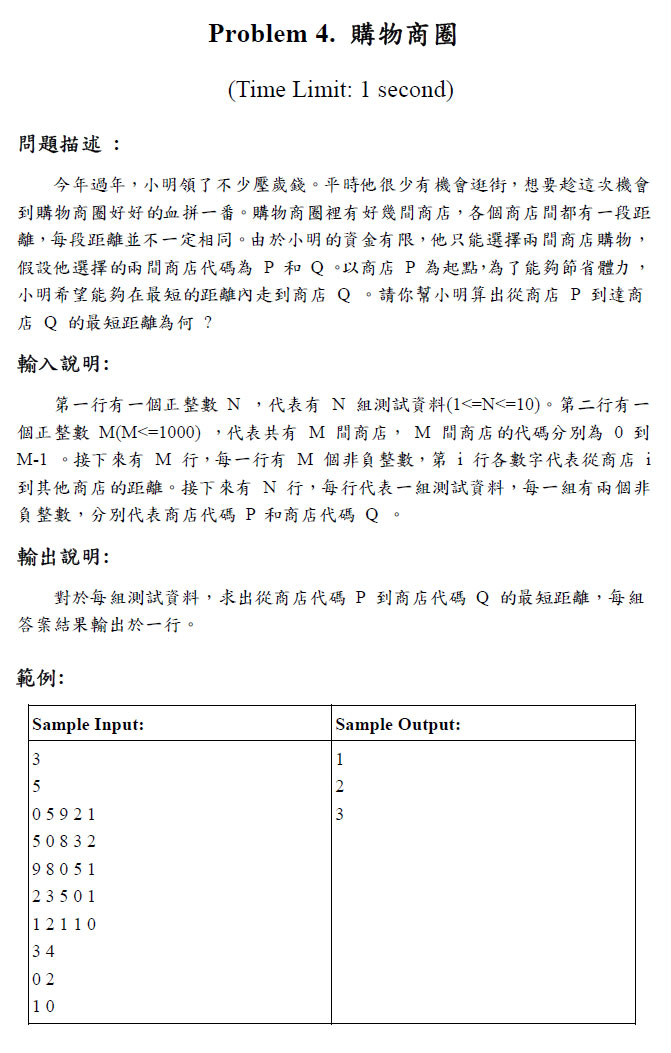
\includegraphics[height=.95\textheight]{../solutions/fig/58ITSA4}}
\subsection{解題思惟}
\begin{enumerate}
	\item m個點之間相互的距離用二維矩陣處理比較容易,因為m不會超過1000,可以宣告一個d[1000][1000]的二維陣列,其中$d_{st}$表示商店s和商店t的距離。
	\item 商店s和商店t的最短途徑要怎麼算呢?我們可以用迭代的方法思考,首先,如果直接從s到t,那麼距離就是$d_{st}$,但如果經過商店$i$,則距離會是
	$d_{si}+d_{it}$,後者有可能會比較短。前者可以看成走一步,後者可以看成走兩步。當然也有可能會有更多步,但距離更短的情況發生。
	\item 我們考慮$s$到所有$i$的最短距離,只走一步的話,就是$d_{si}$,如果走兩步的話,就要檢查所有的$j, j\ne i$,看那一個$j$會使$d_{sj}+d_{ji}$最短。假設找到$j=k$是最好的情況,那我們還要檢查看看$d_{sk}+d_{ki}$有沒有比$d_{si}$更好,如果有的話,表示走兩步的情形,會有比走一步更好的情況發生。
	\item 迭代的方式,就是從一步開始考慮,這時$s$到$i, i\ne s$的最短途徑距離定義成$d_i = d_{si}$。
	\item 接下來我們針對所有多走一步的情況,計算看看有沒有可能找到$j, j\ne s$,使得$d_{sj}+d_{ji}$比$d_i$更小,如果有的話,表示我們找到了多走一步,但距離比較短的方式,那我們就可以更新$d_i$的值。
	\item 只要有一個$d_i$的值被更新了,表示有可能有更好的途徑,我們就重複上一步驟,繼續更新所有的$d_i$。如果已經沒有任何$d_i$可以更新,那表示已經找不到更好的途徑了,那這時候$d_t$就是從$s$到$t$的最短途徑了。
\end{enumerate}

\subsection{程式碼}
\begin{cppcode}
#include <iostream>

using namespace std;

int m, d[1000][1000];

int mindis(int s, int t);

int main()
{
	int kase;
	cin >> kase >> m;
	for (int r=0; r<m; r++) for (int c=0; c<m; c++) cin >> d[r][c];
	while (kase--) {
		int s, t;
		cin >> s >> t;
		cout << mindis(s, t) << endl;
	}
	return 0;
}

int mindis(int s, int t)
{
	int dis[1000];
	for (int i=0; i<m; i++) dis[i] = d[s][i];
	bool change;
	do {
		change = false;
		for (int i=0; i<m; i++) {
			if (i==s) continue;
			for (int j=0; j<m; j++) {
				if (j==s) continue;
				if (dis[j]+d[j][i] < dis[i]) { dis[i]=dis[j]+d[j][i]; change=true; }
			}
		}
	} while (change);
	return dis[t];
}
\end{cppcode}
\newpage
\section{ITSA-58-5 Set Partition}
\centerline{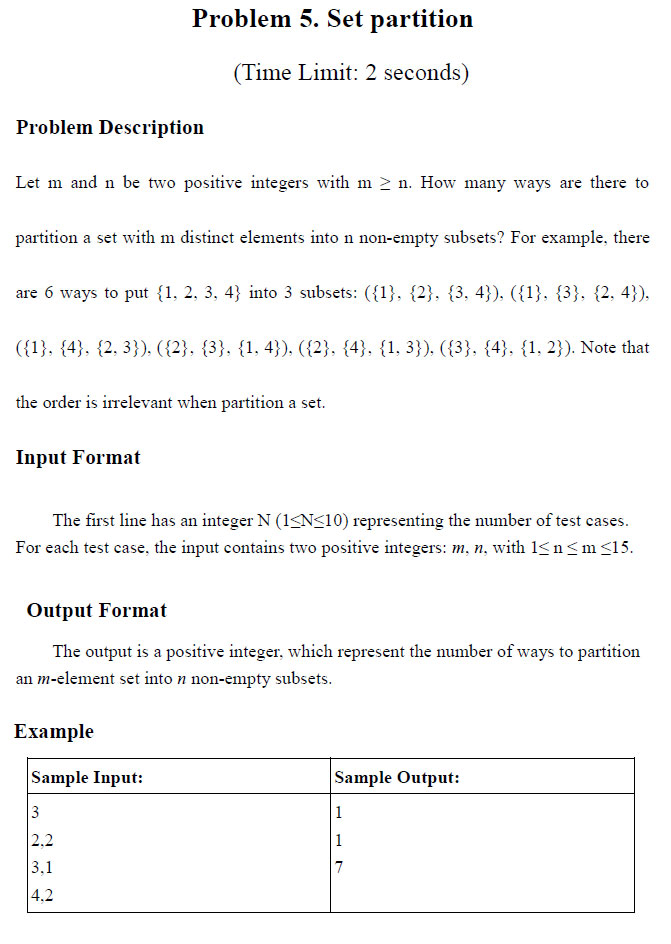
\includegraphics[height=.95\textheight]{../solutions/fig/58ITSA5}}

\subsection{解題思惟}
\begin{enumerate}
	\item 這一題要直接找到公式計算的話,看起來挺困難的。不過使用遞迴的角度去思考,會發現並沒有那麼難。
	\item 假設m個數字$1,2,\cdots,m$分成n堆的所有可能數目是f(m,n)。現在我們先把1拿出來單獨考慮,這時只有兩種情況,一種是1自己一堆,另一種是1跟其他數字一堆。
	\item 如果1自己一堆的話,那麼剩下的堆數是n-1,而且只有m-1個數,所以總共的可能數目會是f(m-1, n-1)。
	\item 如果1跟別人一堆的話,那麼先不考慮1,就是m-1個數有n堆,所以可能的數目會是f(m-1, n)。接著考慮1會放在哪一堆呢?放哪一堆都有可能,也就是有n種放法。這樣的話,總共的可能數目變成$n\times f(m-1, n)$。這裡面會不會有重複的情況發生呢?如果有兩種分法是相等的,那麼1的那堆數字要相同,其他的n-1堆不管順序的也要相同,那把1拿掉,這兩種分法等於也是相同的,但我們所用的f(m-1, n)的定義,就是不同的分法,所以就違反我們的假設了,因此不會有重複的情況發生。
	\item 根據以上的分析,我們已經找到遞迴的規則。接下來要找終止條件,這個比較容易,就是當n=1的時候,表示只有一堆,也只有一種分法;當n=m的時候,表示分成m堆,等於每個數各自一堆,也只有一種分法。
\end{enumerate}

\subsection{程式碼}
\begin{cppcode}
#include <iostream>

using namespace std;

int f(int m, int n);

int main()
{
	int kase, m, n;
	cin >> kase;
	while (kase--) {
		char c;
		cin >> m >> c >> n;
		cout << f(m, n) << endl;
	}
	return 0;
}

int f(int m, int n)
{
	if (n==1 || n==m) return 1;
	return f(m-1, n-1) + n*f(m-1, n);
}
\end{cppcode}

\end{document}
